\documentclass[11pt]{article} \usepackage{graphicx}  \textwidth = 6.5 in \textheight = 9 in \oddsidemargin = 0.0 in \evensidemargin = 0.0 in \topmargin = 0.0 in \headheight = 0.0 in \headsep = 0.0 in \parskip = 0.2in \parindent = 0.0in   \newlength{\nameraise} \setlength{\nameraise}{.07in}  \newlength{\nameoverhang} \setlength{\nameoverhang}{.22in}   \begin{document}  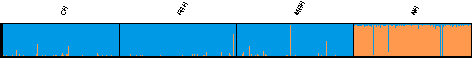
\includegraphics[width=6.5 in, scale=0.9]{./final_pdf//BB_ds_Clumped_TopLabel_k002r001.pdf}~\hspace*{-\nameoverhang}\raisebox{\nameraise}{} \\
Distruct Plots at $K=2$.












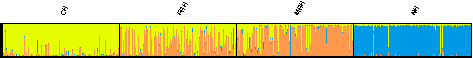
\includegraphics[width=6.5 in, scale=0.9]{./final_pdf//BB_ds_Clumped_TopLabel_k003r001.pdf}~\hspace*{-\nameoverhang}\raisebox{\nameraise}{} \\
Distruct Plots at $K=3$.












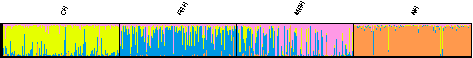
\includegraphics[width=6.5 in, scale=0.9]{./final_pdf//BB_ds_Clumped_TopLabel_k004r001.pdf}~\hspace*{-\nameoverhang}\raisebox{\nameraise}{} \\
Distruct Plots at $K=4$.





\end{document}
